%!TEX TS-program = pdflatex
%!TEX root = tesi.tex
%!TEX encoding = UTF-8 Unicode

% in figura~\ref{fig:p1_overview}.
%\begin{figure}[ht]
%  \begin{center}
%    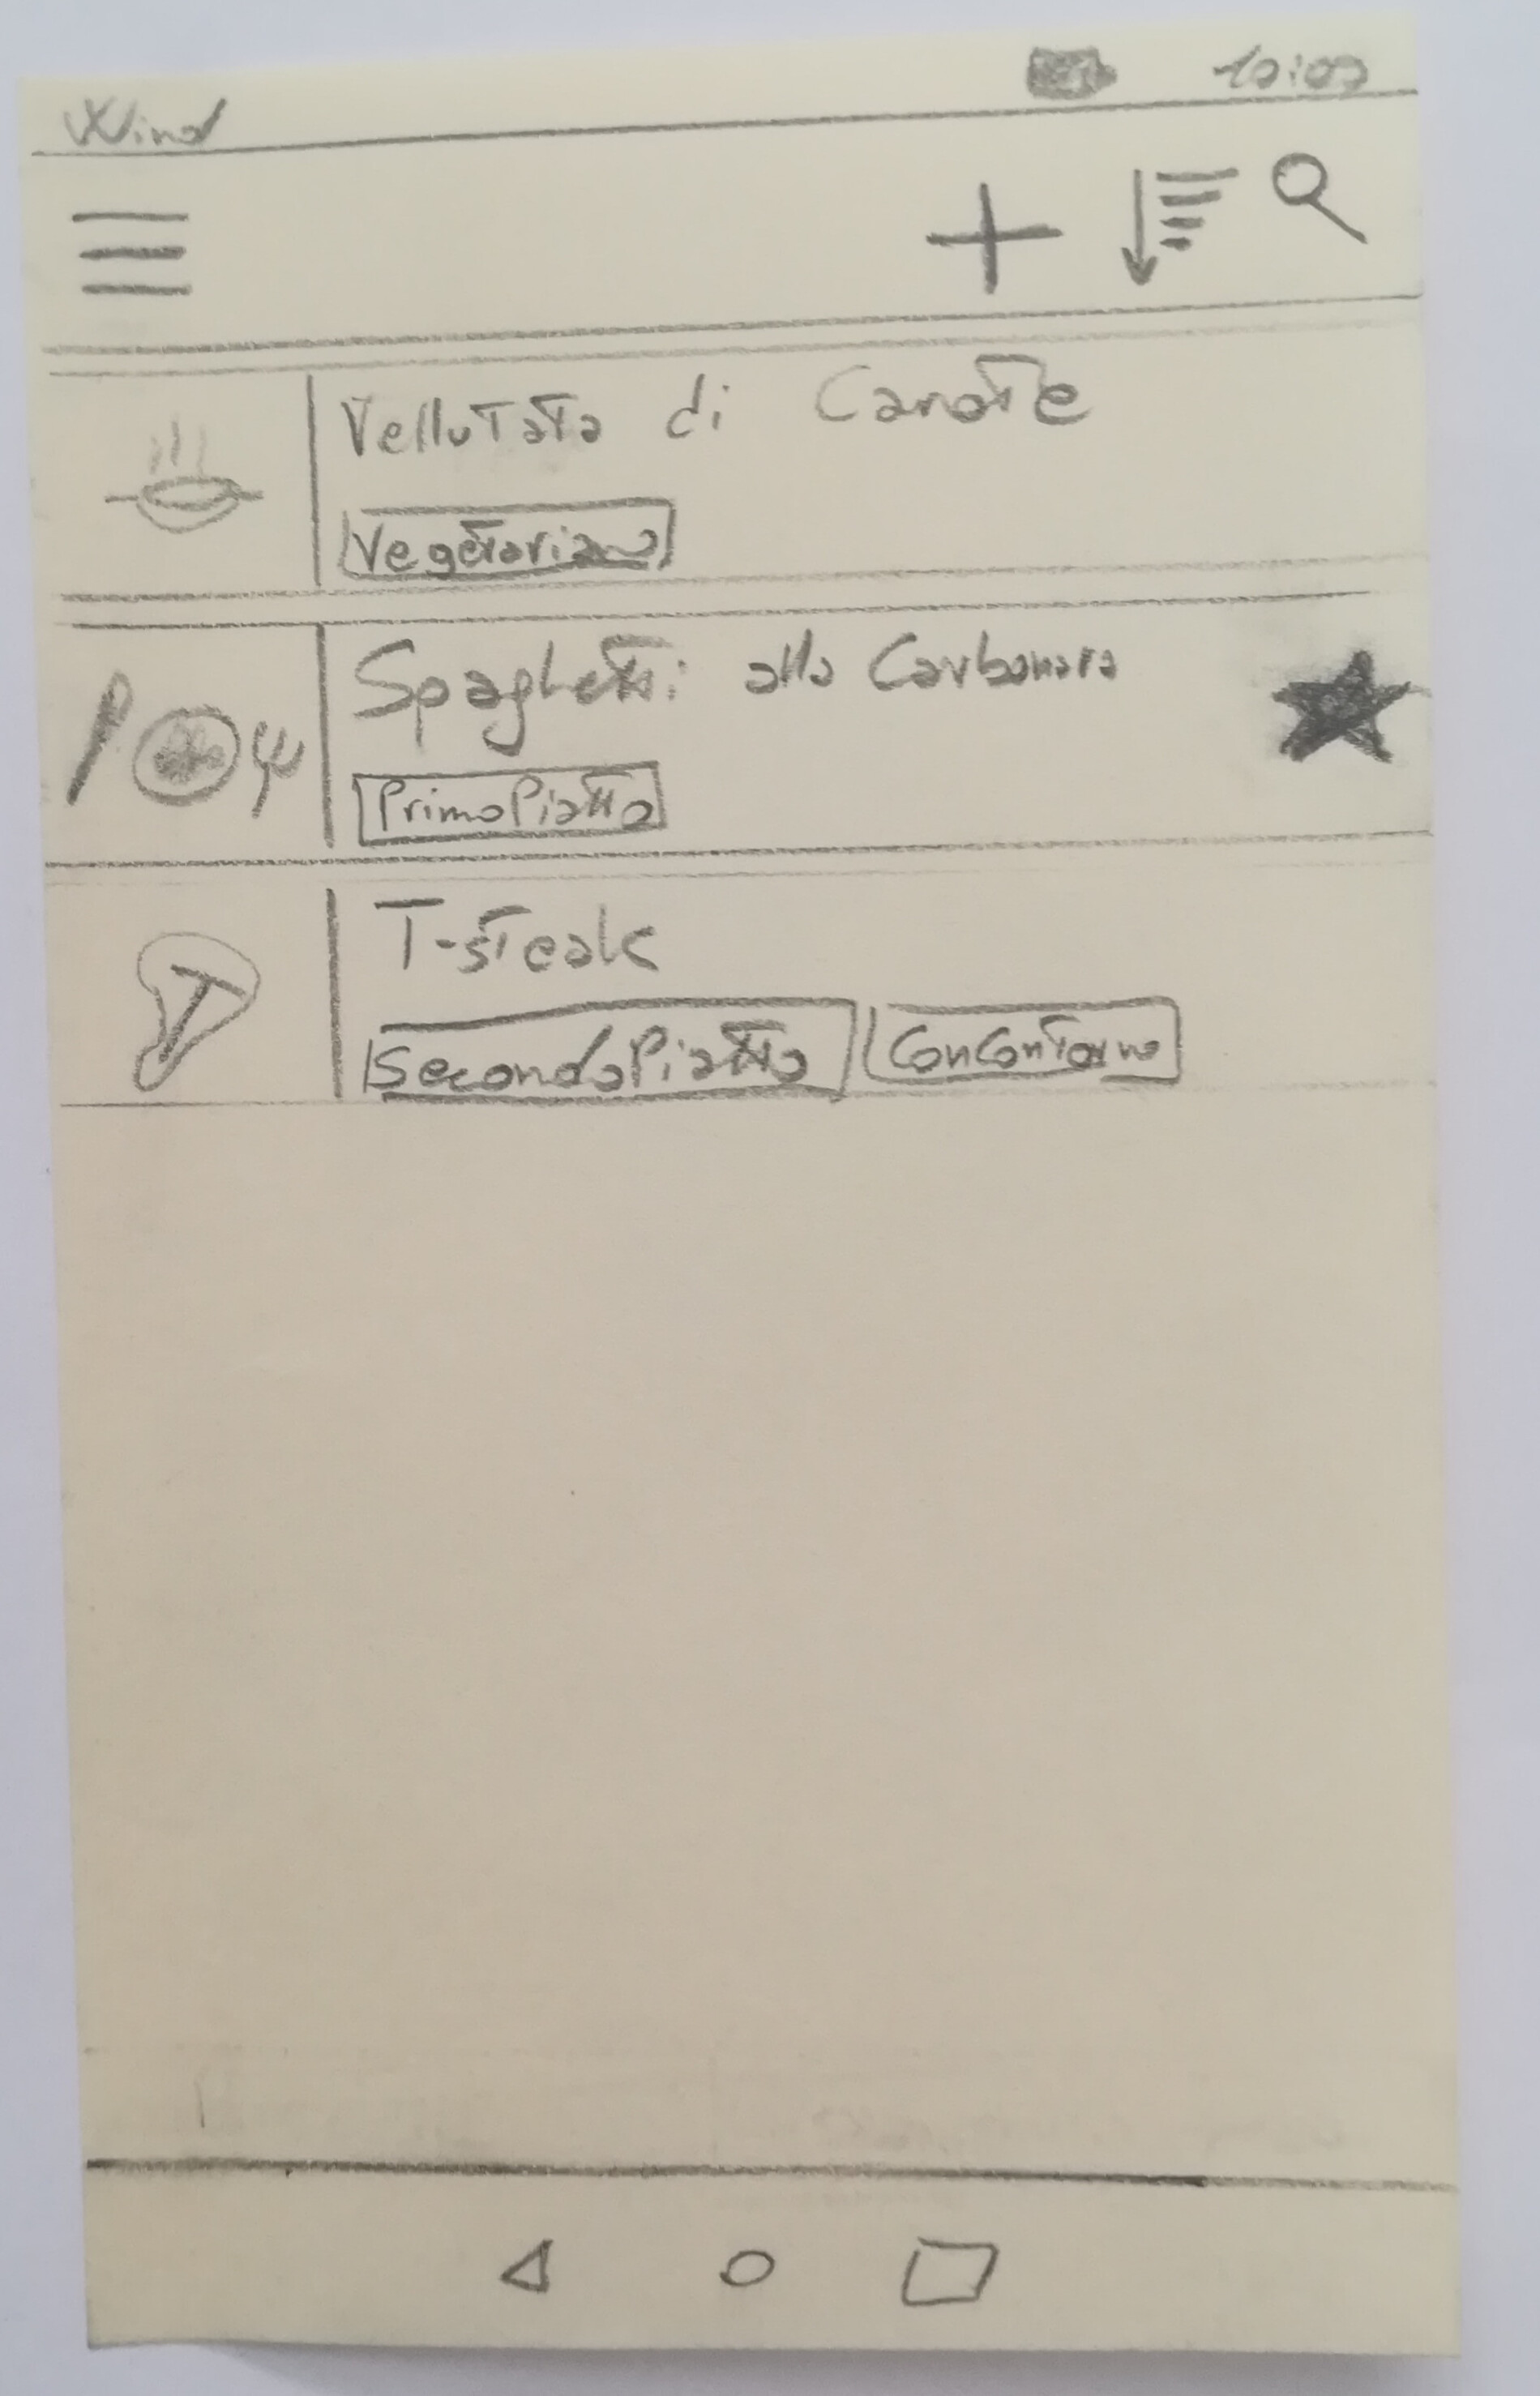
\includegraphics[width=0.6\textwidth]{prototipo1/main_ricette_lista_tags}
%    \caption{Primo storyboard}
%    \label{fig:roa}
%  \end{center}
%\end{figure}

% cuciamo_a
% cuciamo_b
% cuciamo_c
% edit_ricetta_ingredienti
% edit_ricetta_preparazione
% edit_ricetta_riepilogo
% 
% main_ricette_lista_cards
% main_ricette_lista_tags_fab
% main_ricette_lista_tags






\section{Secondo Assignment}

\subsection{Primo Prototipo Low-Fidelity}

%Il risultato di una prima prototipizzazione è riportato in figura~\ref{fig:p1_overview}.
%Come si può 
%
%\begin{figure}[ht]
%  \begin{center}
%    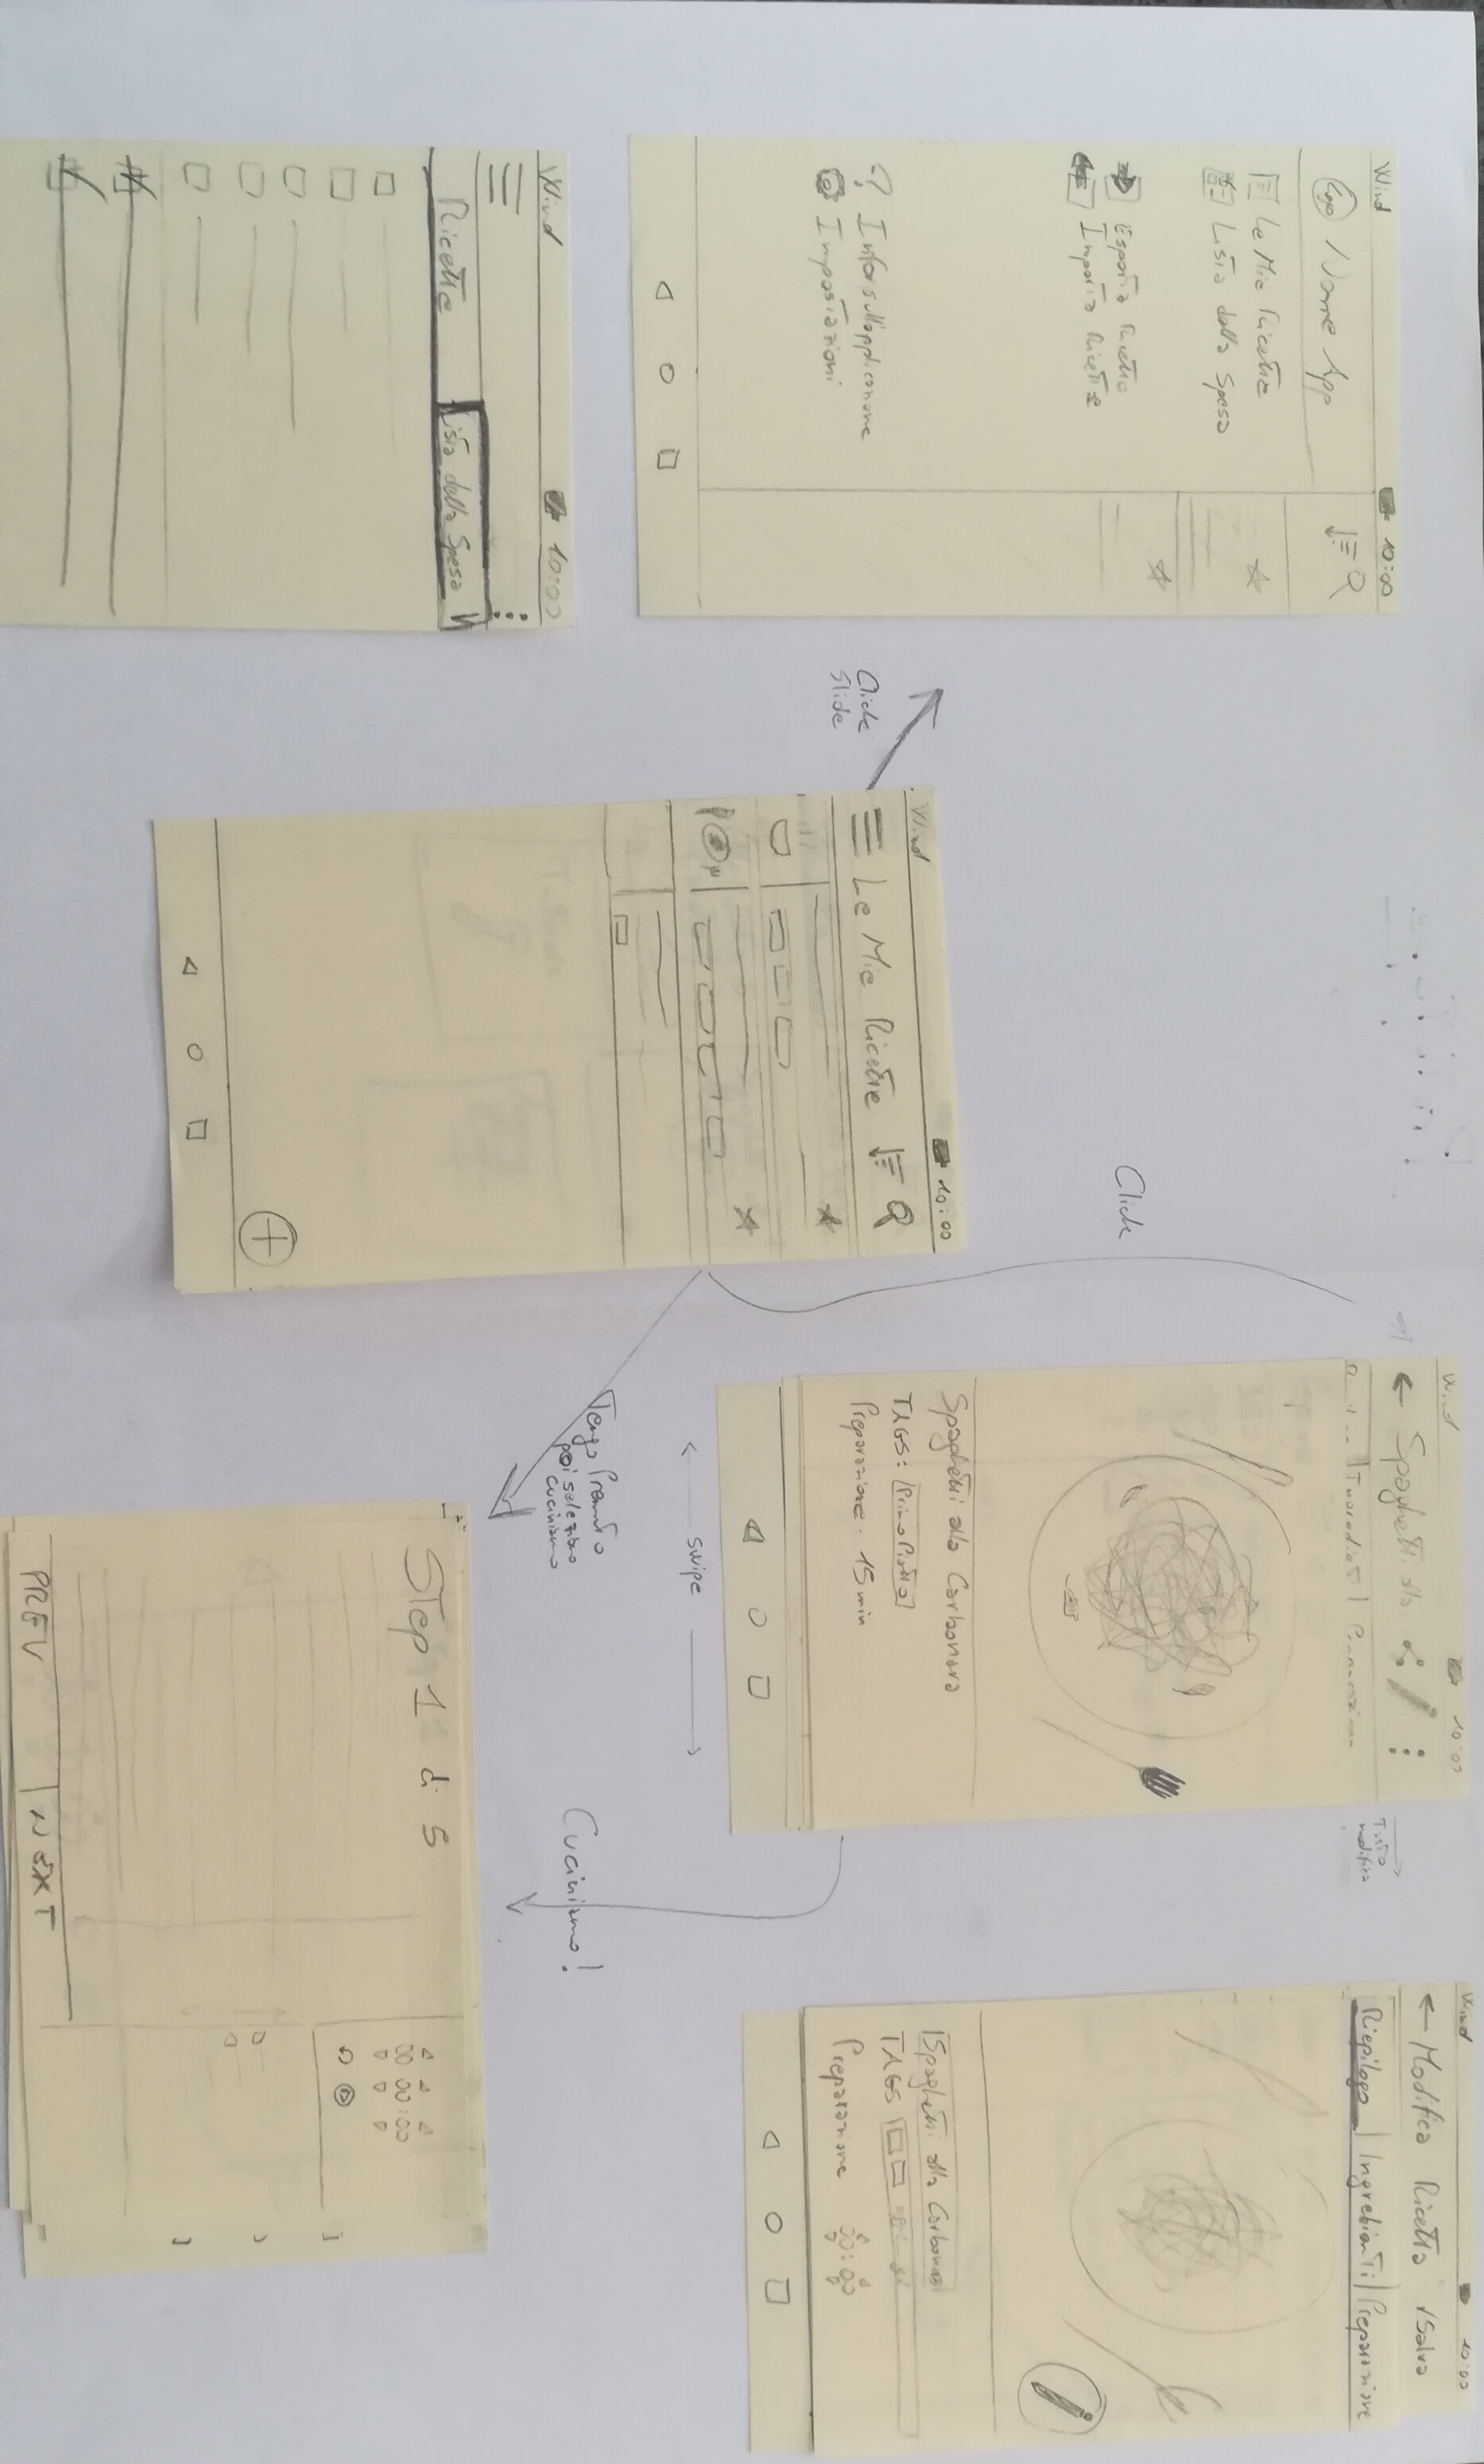
\includegraphics[width=0.6\textwidth, angle=90]{prototipo1/overview}
%    \caption{Primo storyboard}
%    \label{fig:p1_overview}
%  \end{center}
%\end{figure}

In figura~\ref{fig:p1_main} è riportata la schermata principale dell'applicazione.
Le ricette vengono mostrate in una lista, ogni elemento mostra l'immagine associata alla ricetta, il suo titolo, eventuali etichette (ad esempio primo piatto, secondo piatto, vegetariano, contorno, \dots ) e se la ricetta appartiene ai preferiti.
I tasti in alto a sinistra indicano la possibilità di aggiungere una nuova ricetta, ordinare le ricette oppure cercarne una.

\begin{figure}[ht]
  \begin{center}
    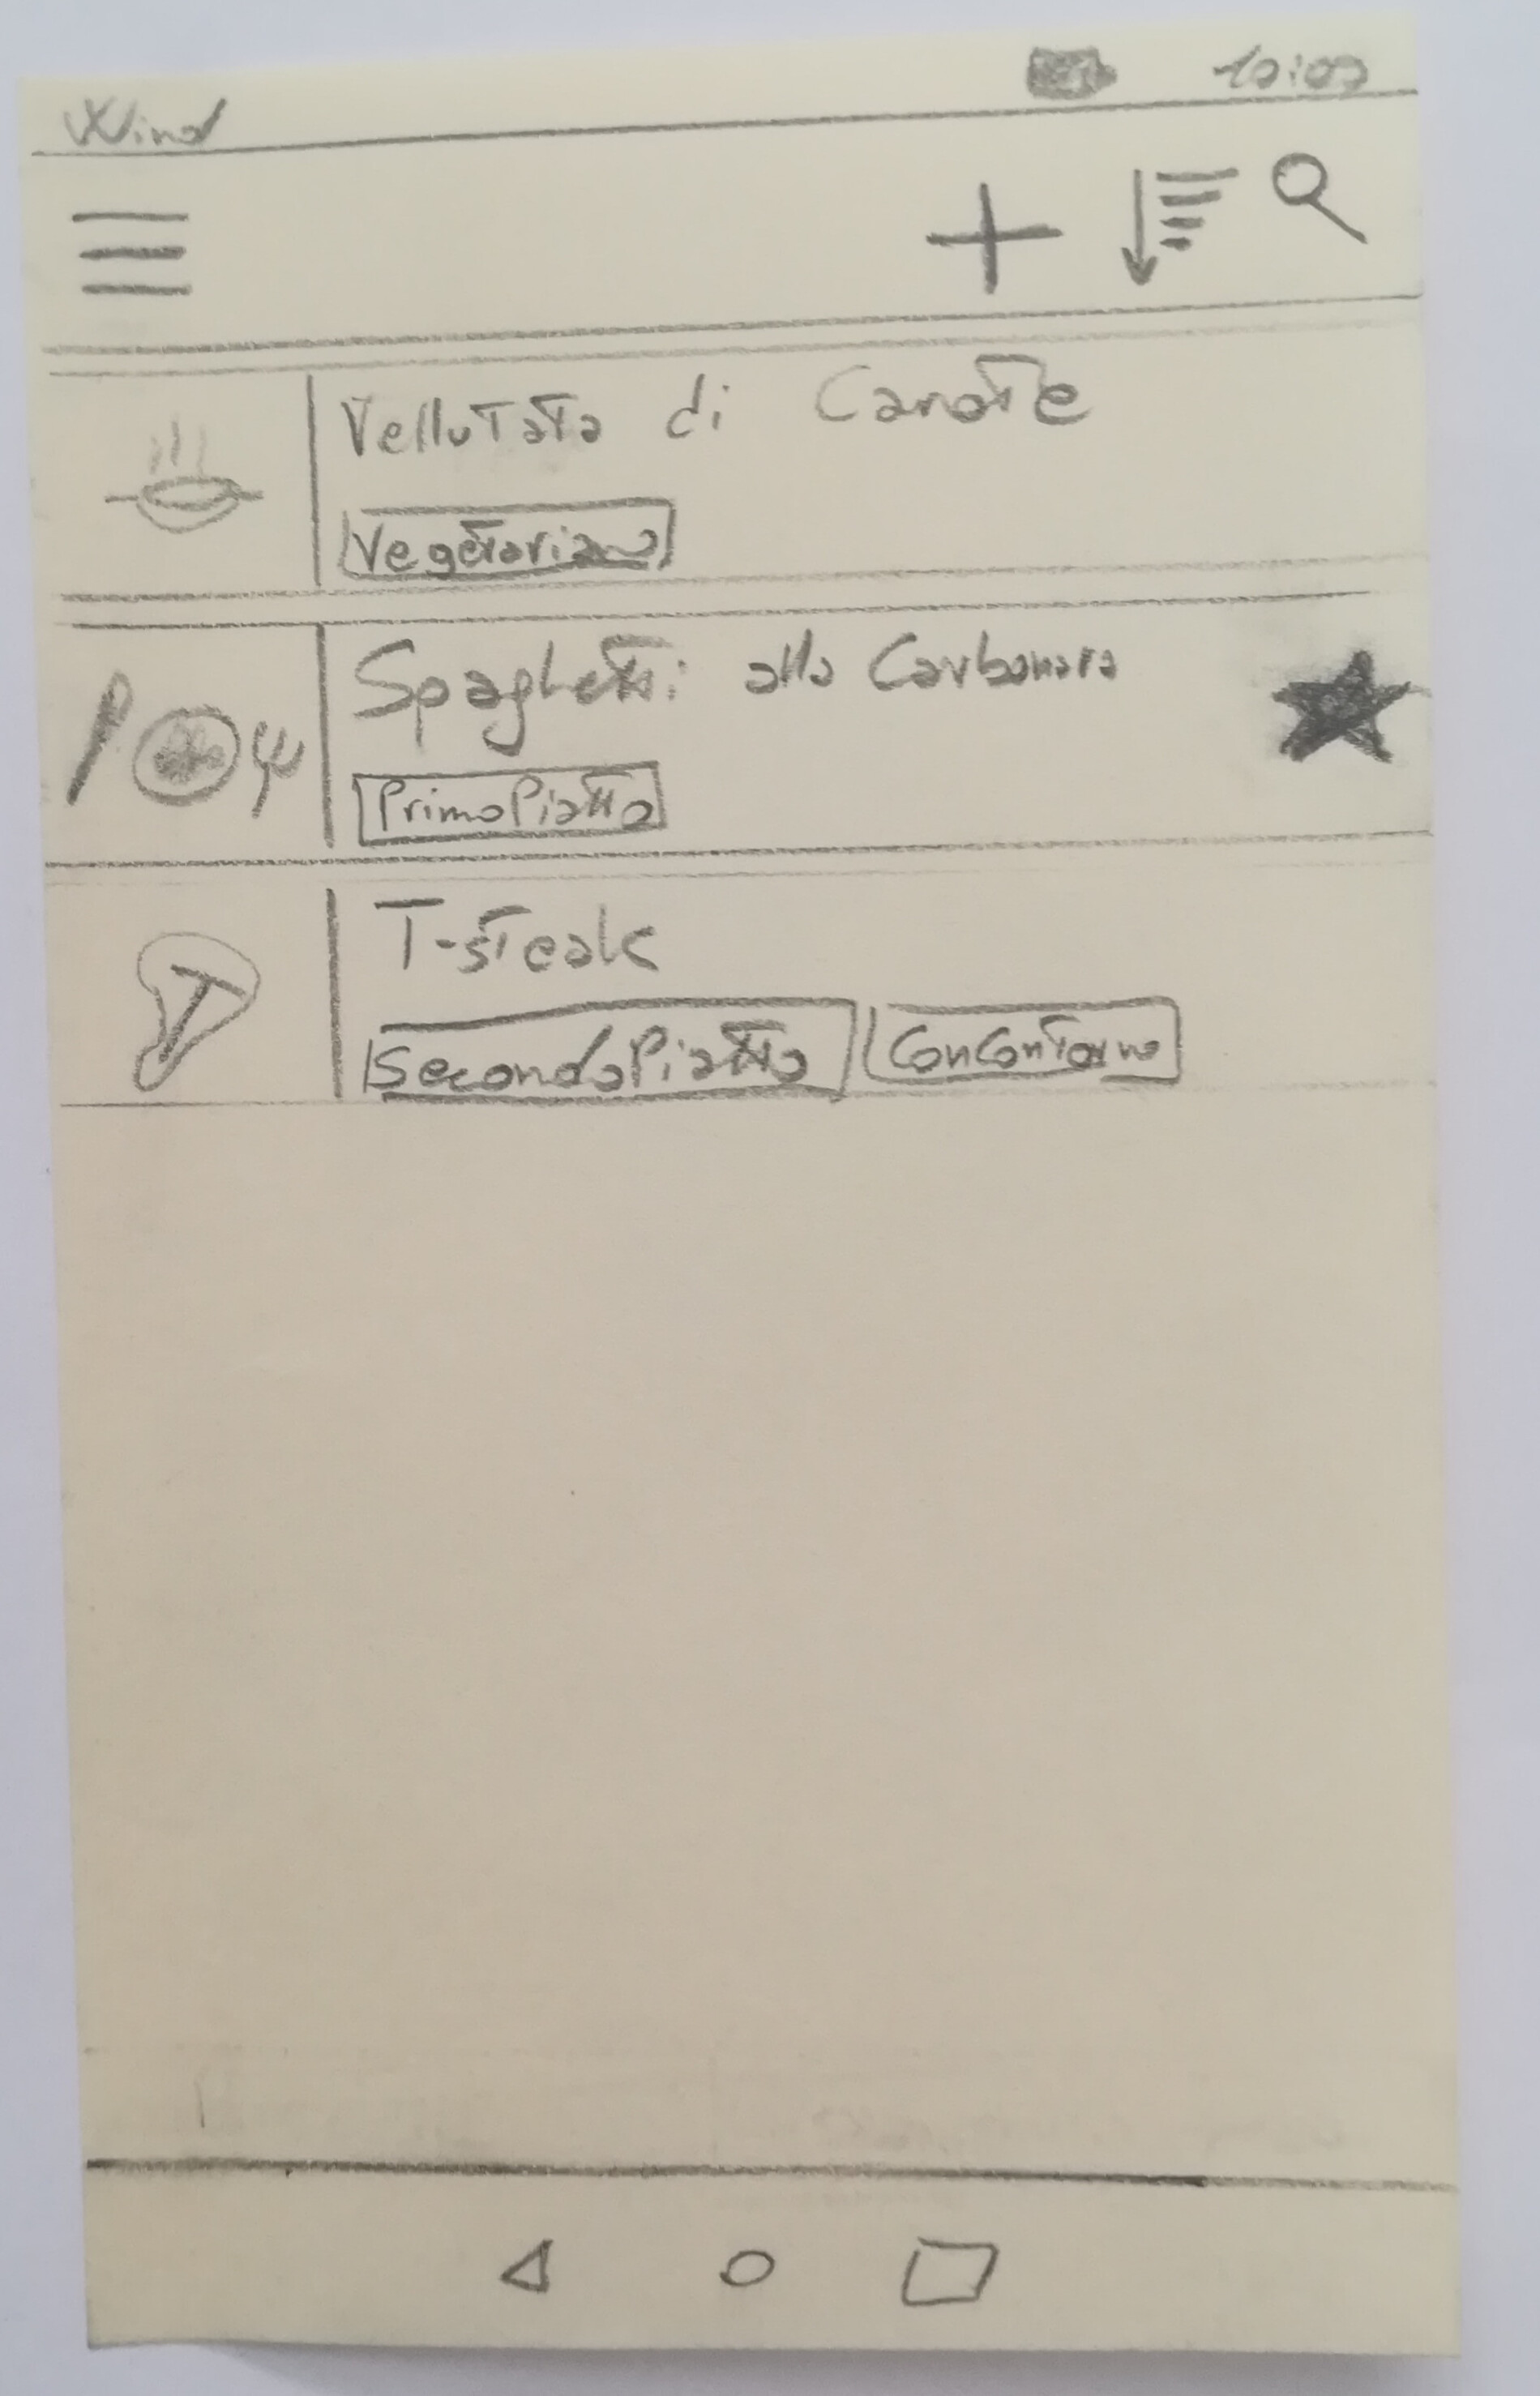
\includegraphics[width=0.6\textwidth]{prototipo1/main_ricette_lista_tags}
    \caption{Schermata principale}
    \label{fig:p1_main}
  \end{center}
\end{figure}

Premendo il tasto in alto a sinistra si apre una TODO laterale, riportata a sinistra in figura \ref{fig:p1_lista_spesa}.
Qui è possibile effettuare varie operazioni, tra cui visualizzare la lista della spesa.
Quest'ultima è divisa in due sezioni in modo che risulti chiaro quali sono gli ingredienti ancora da comprare e quali invece sono già stati acquistati.

\begin{figure}[ht]
  \begin{center}
    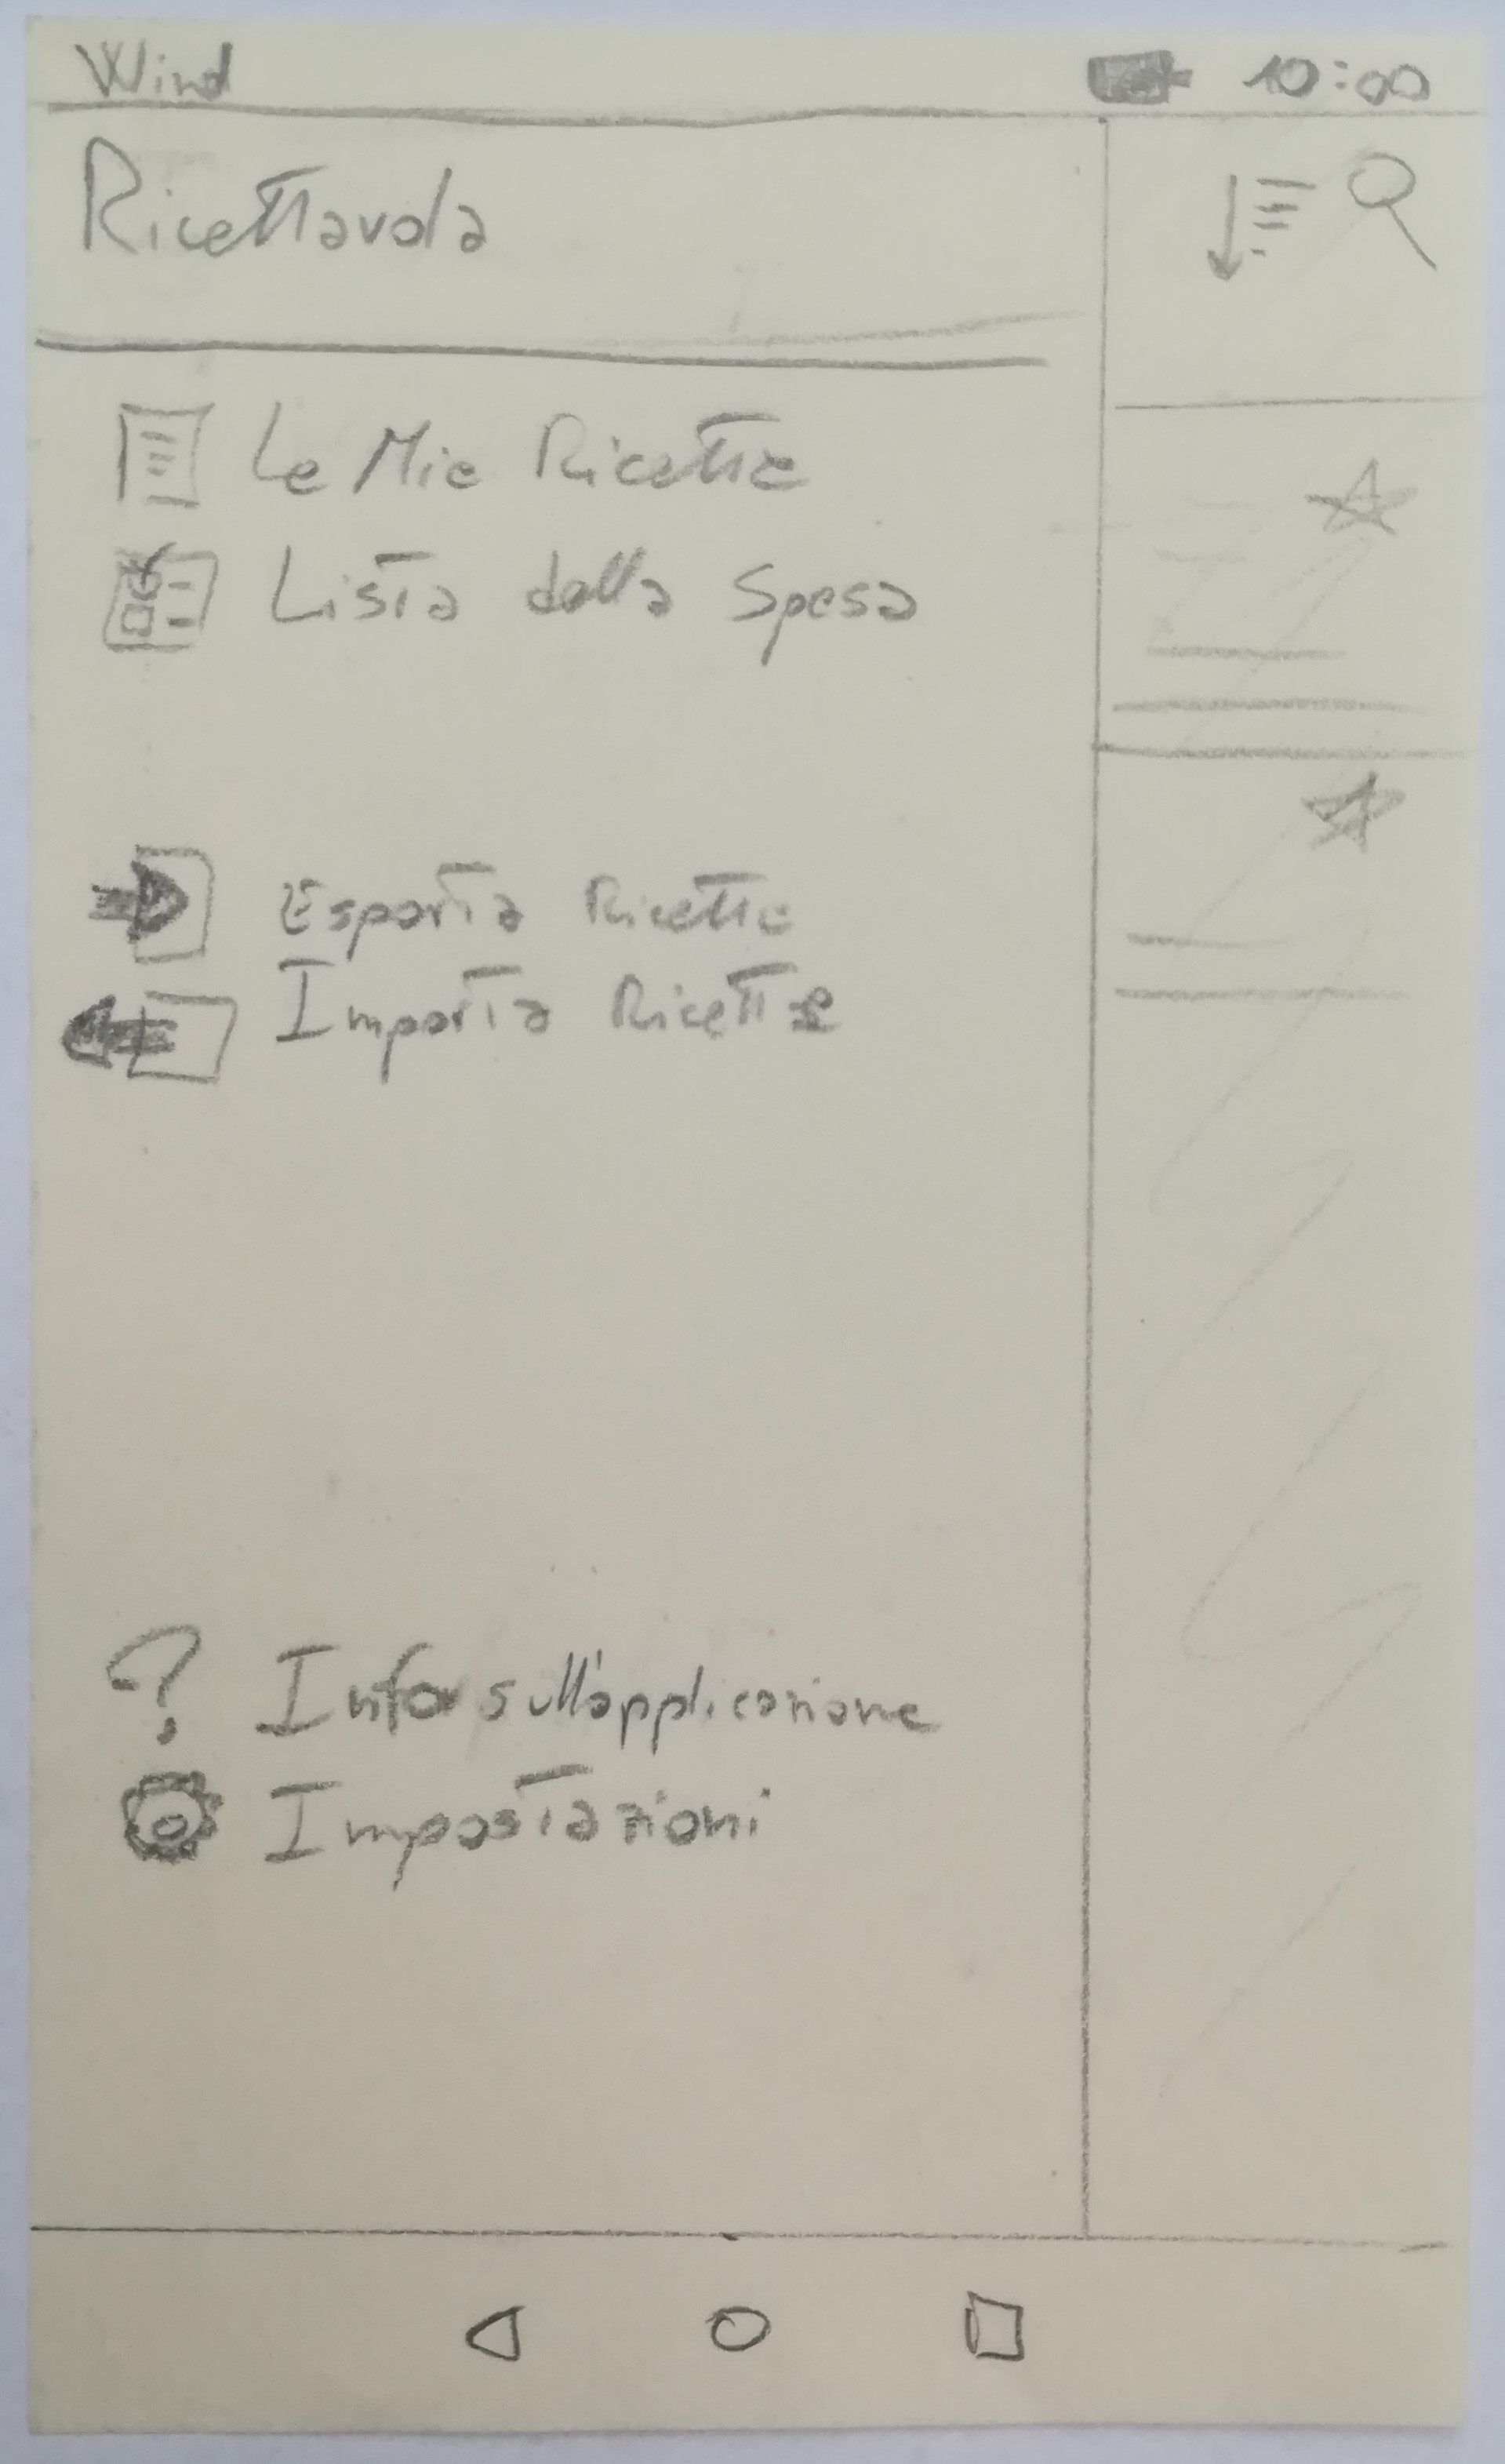
\includegraphics[width=0.4\textwidth]{prototipo1/res1900x3100/tab_laterale}
    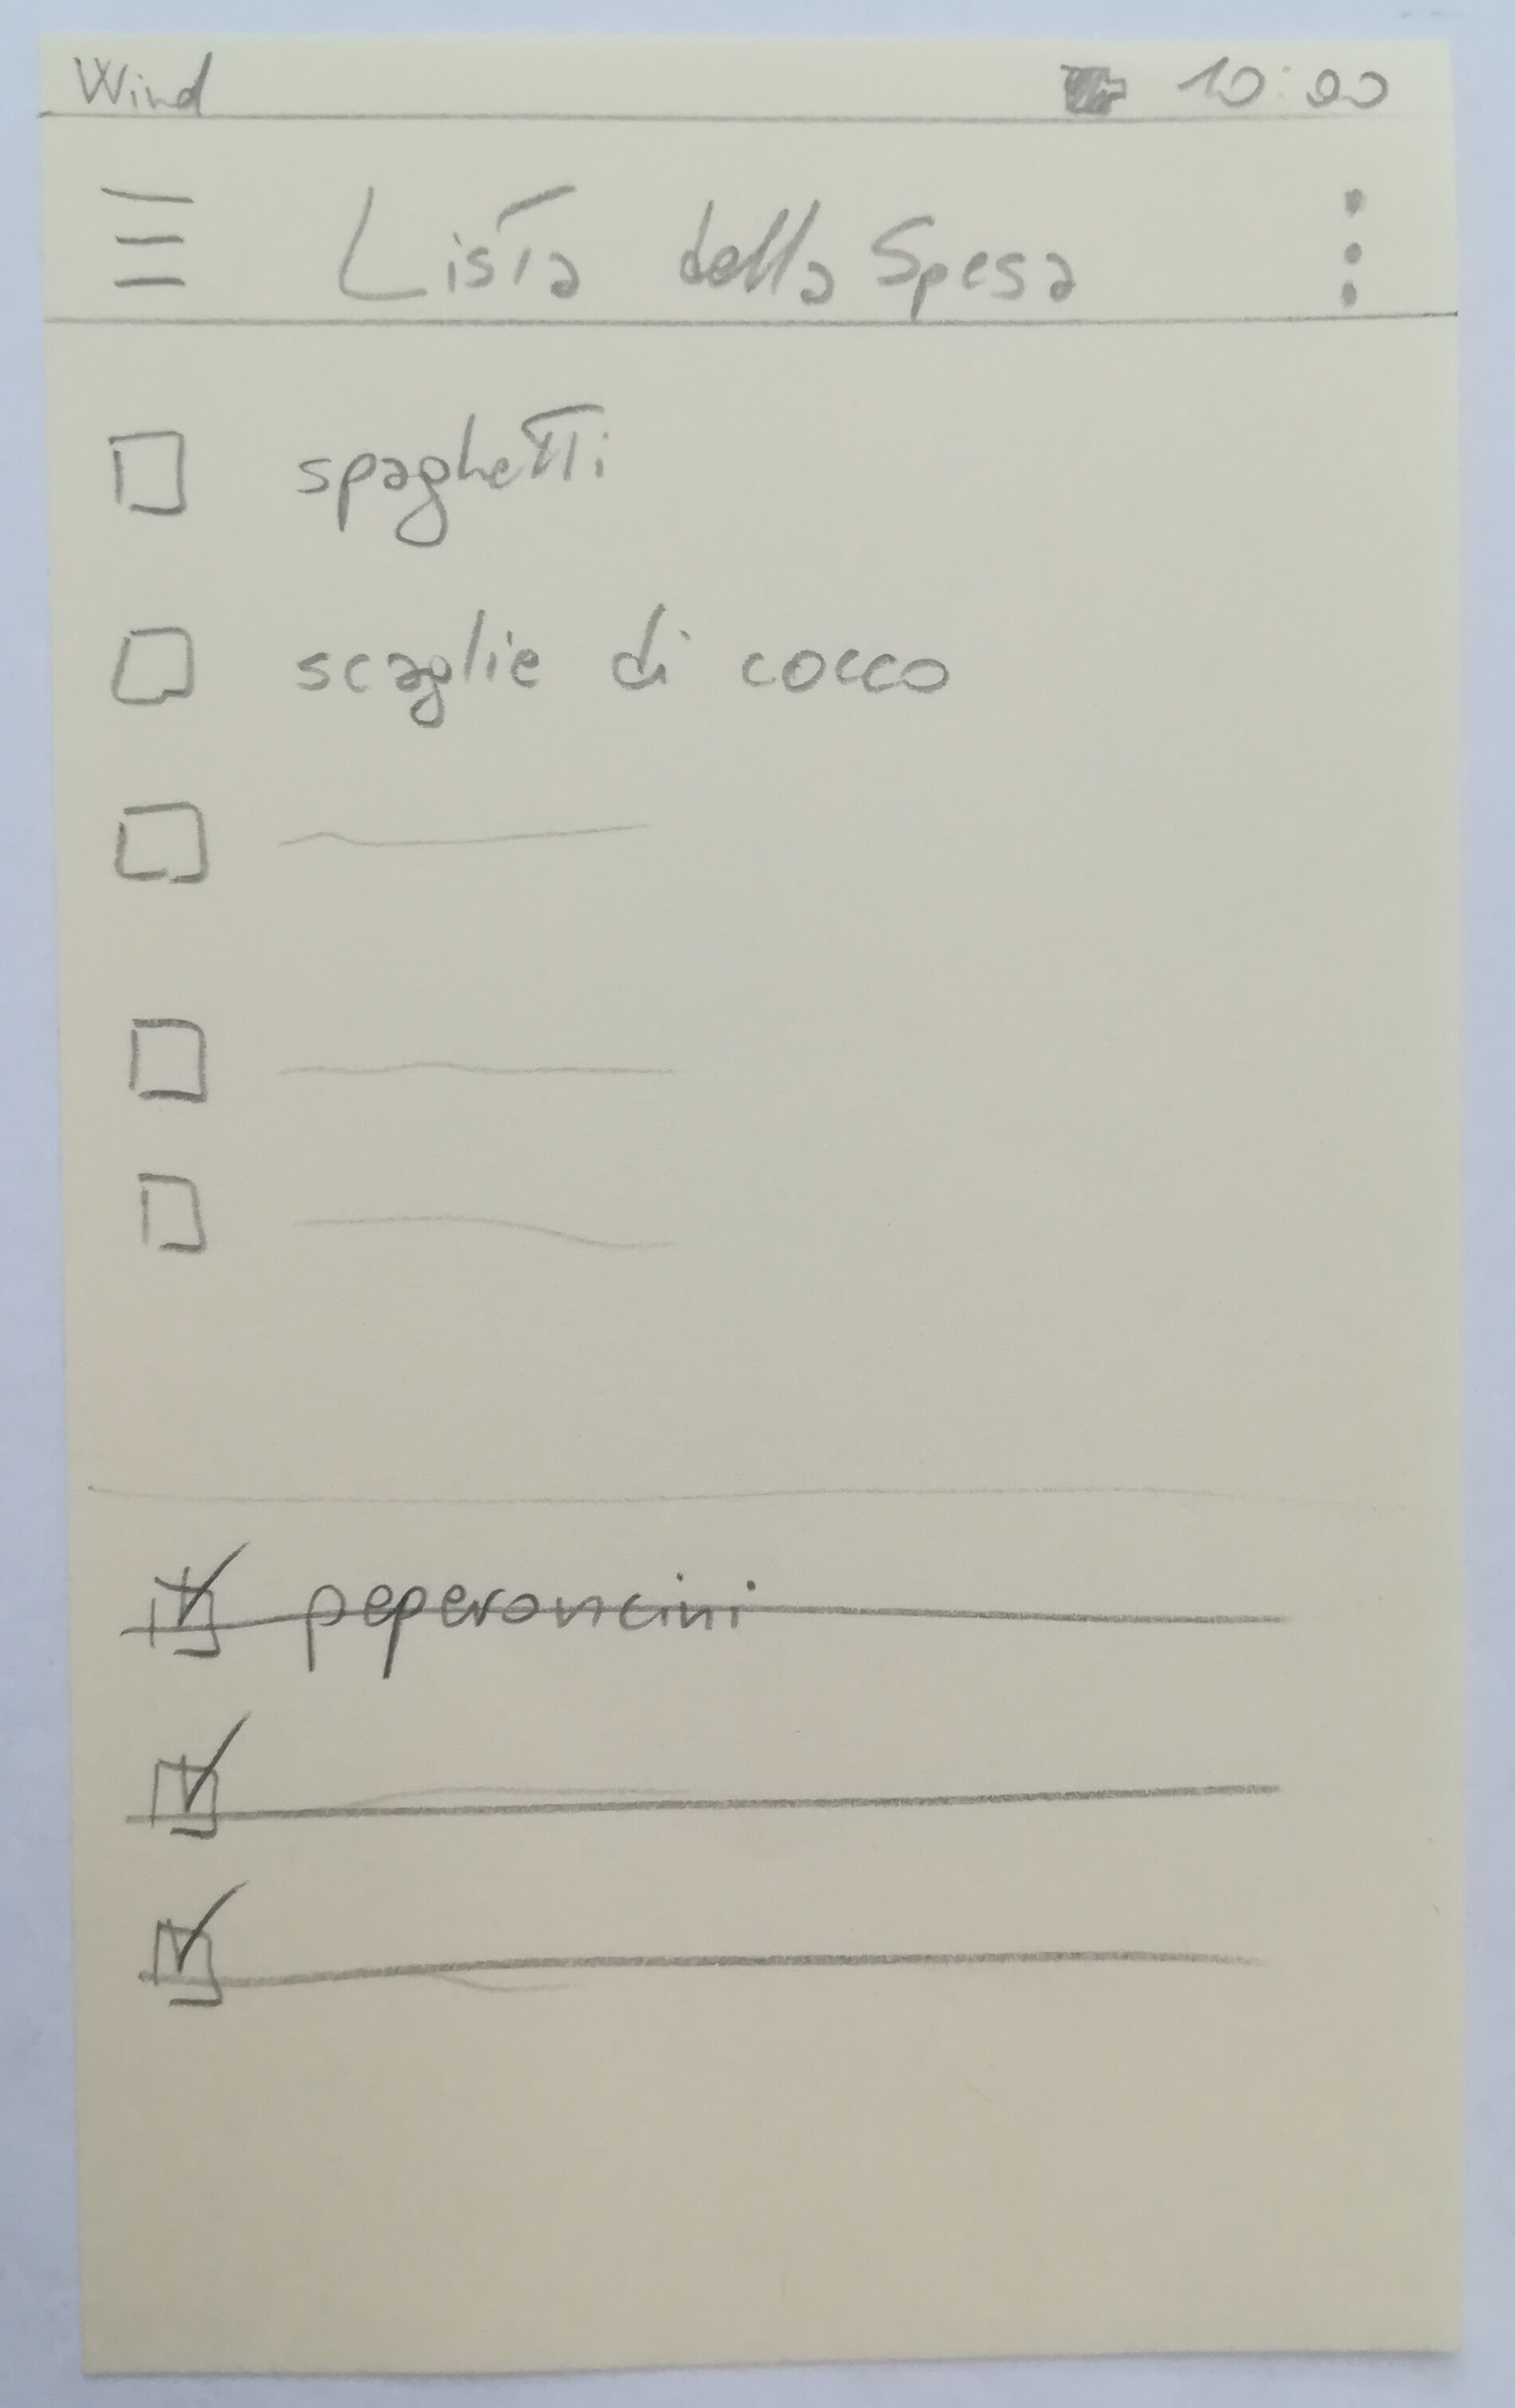
\includegraphics[width=0.4\textwidth]{prototipo1/res1900x3100/main_lista_della_spesa}
    \caption{Da sinistra a destra: TODO laterale, la lista della spesa}
    \label{fig:p1_lista_spesa}
  \end{center}
\end{figure}


Dalla attività principale, premendo una ricetta, si passa alle prima schermata in figura \ref{fig:p1_ricetta}.
Nel toolbar sono presenti alcune azioni comuni, come modificare o condividere la ricetta, e ovviamente la possibilità di tornare alla schermata precedetene.
Poco sotto il toolbar sono presenti tre tab: Riepilogo, Ingredienti, Preparazione.
La prima linguetta è selezionata, infatti si possono osservare le principali informazioni della ricetta selezionata.
Premendo su una linguetta o con un'azione di \texit{swipe} si può passare alle altre schermate.
La seconda immagine mostra

\begin{figure}[ht]
  \begin{center}
    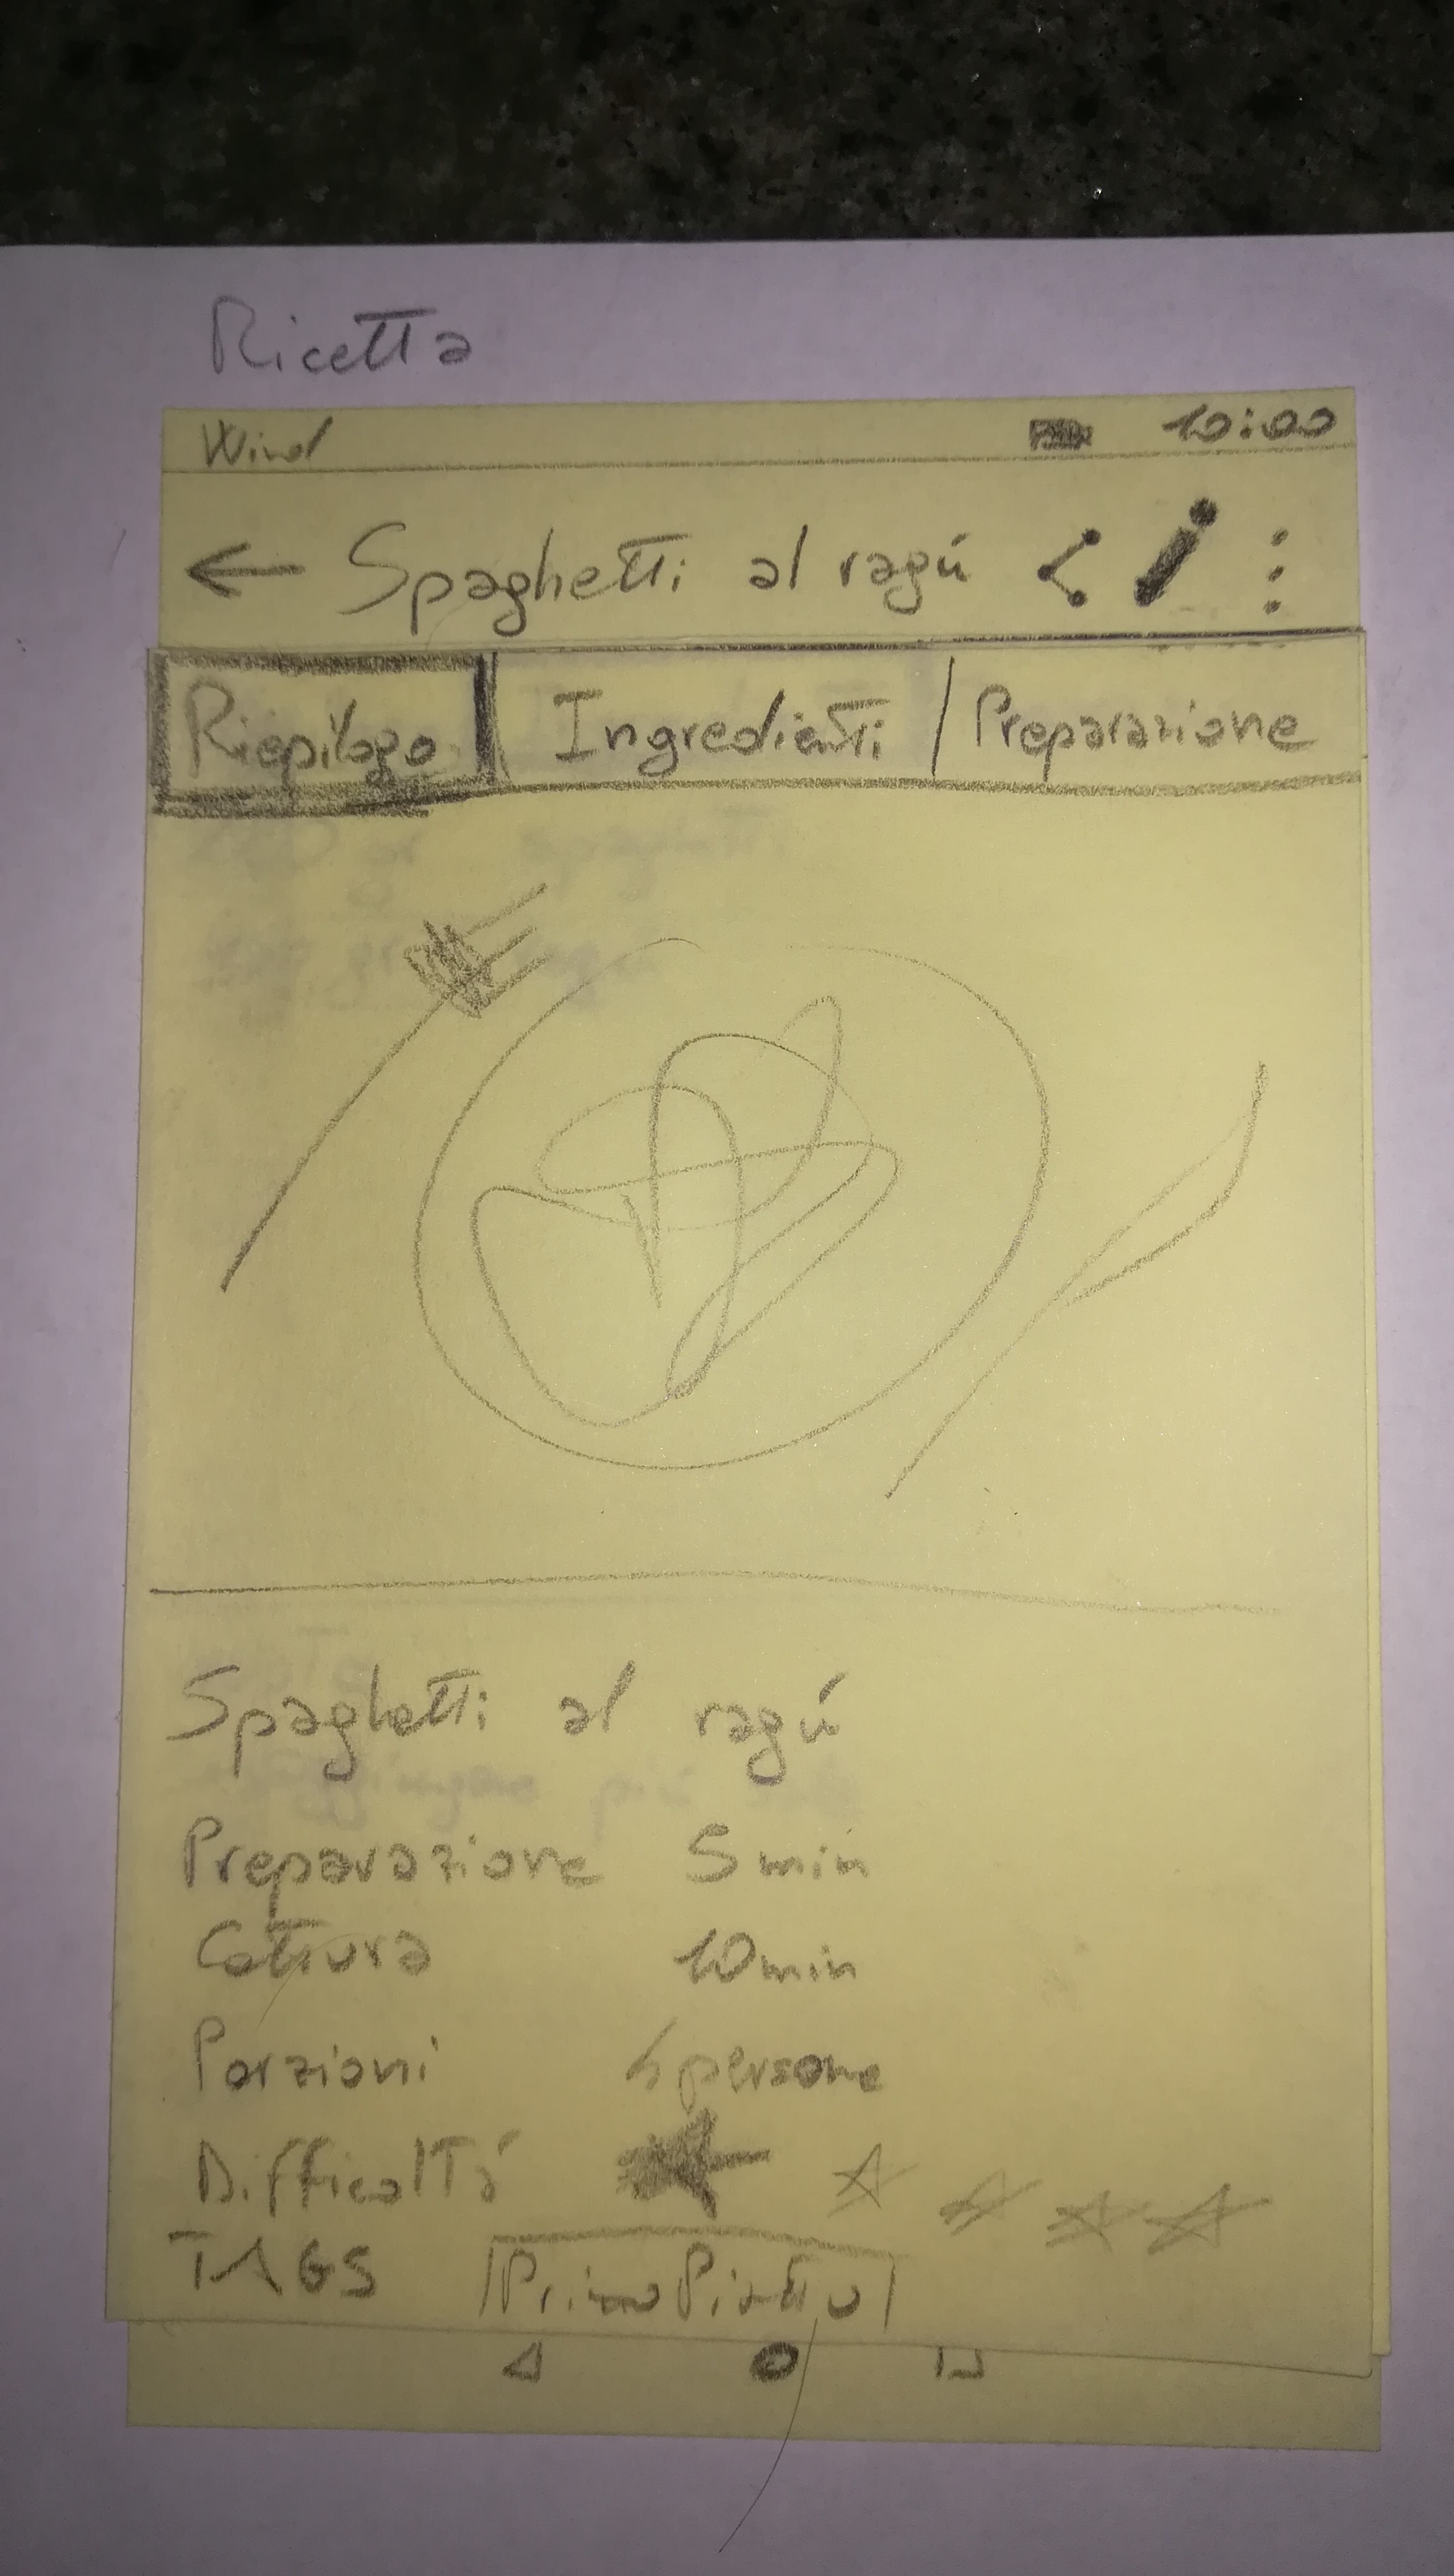
\includegraphics[width=0.4\textwidth]{prototipo1/ricetta_riepilogo}
    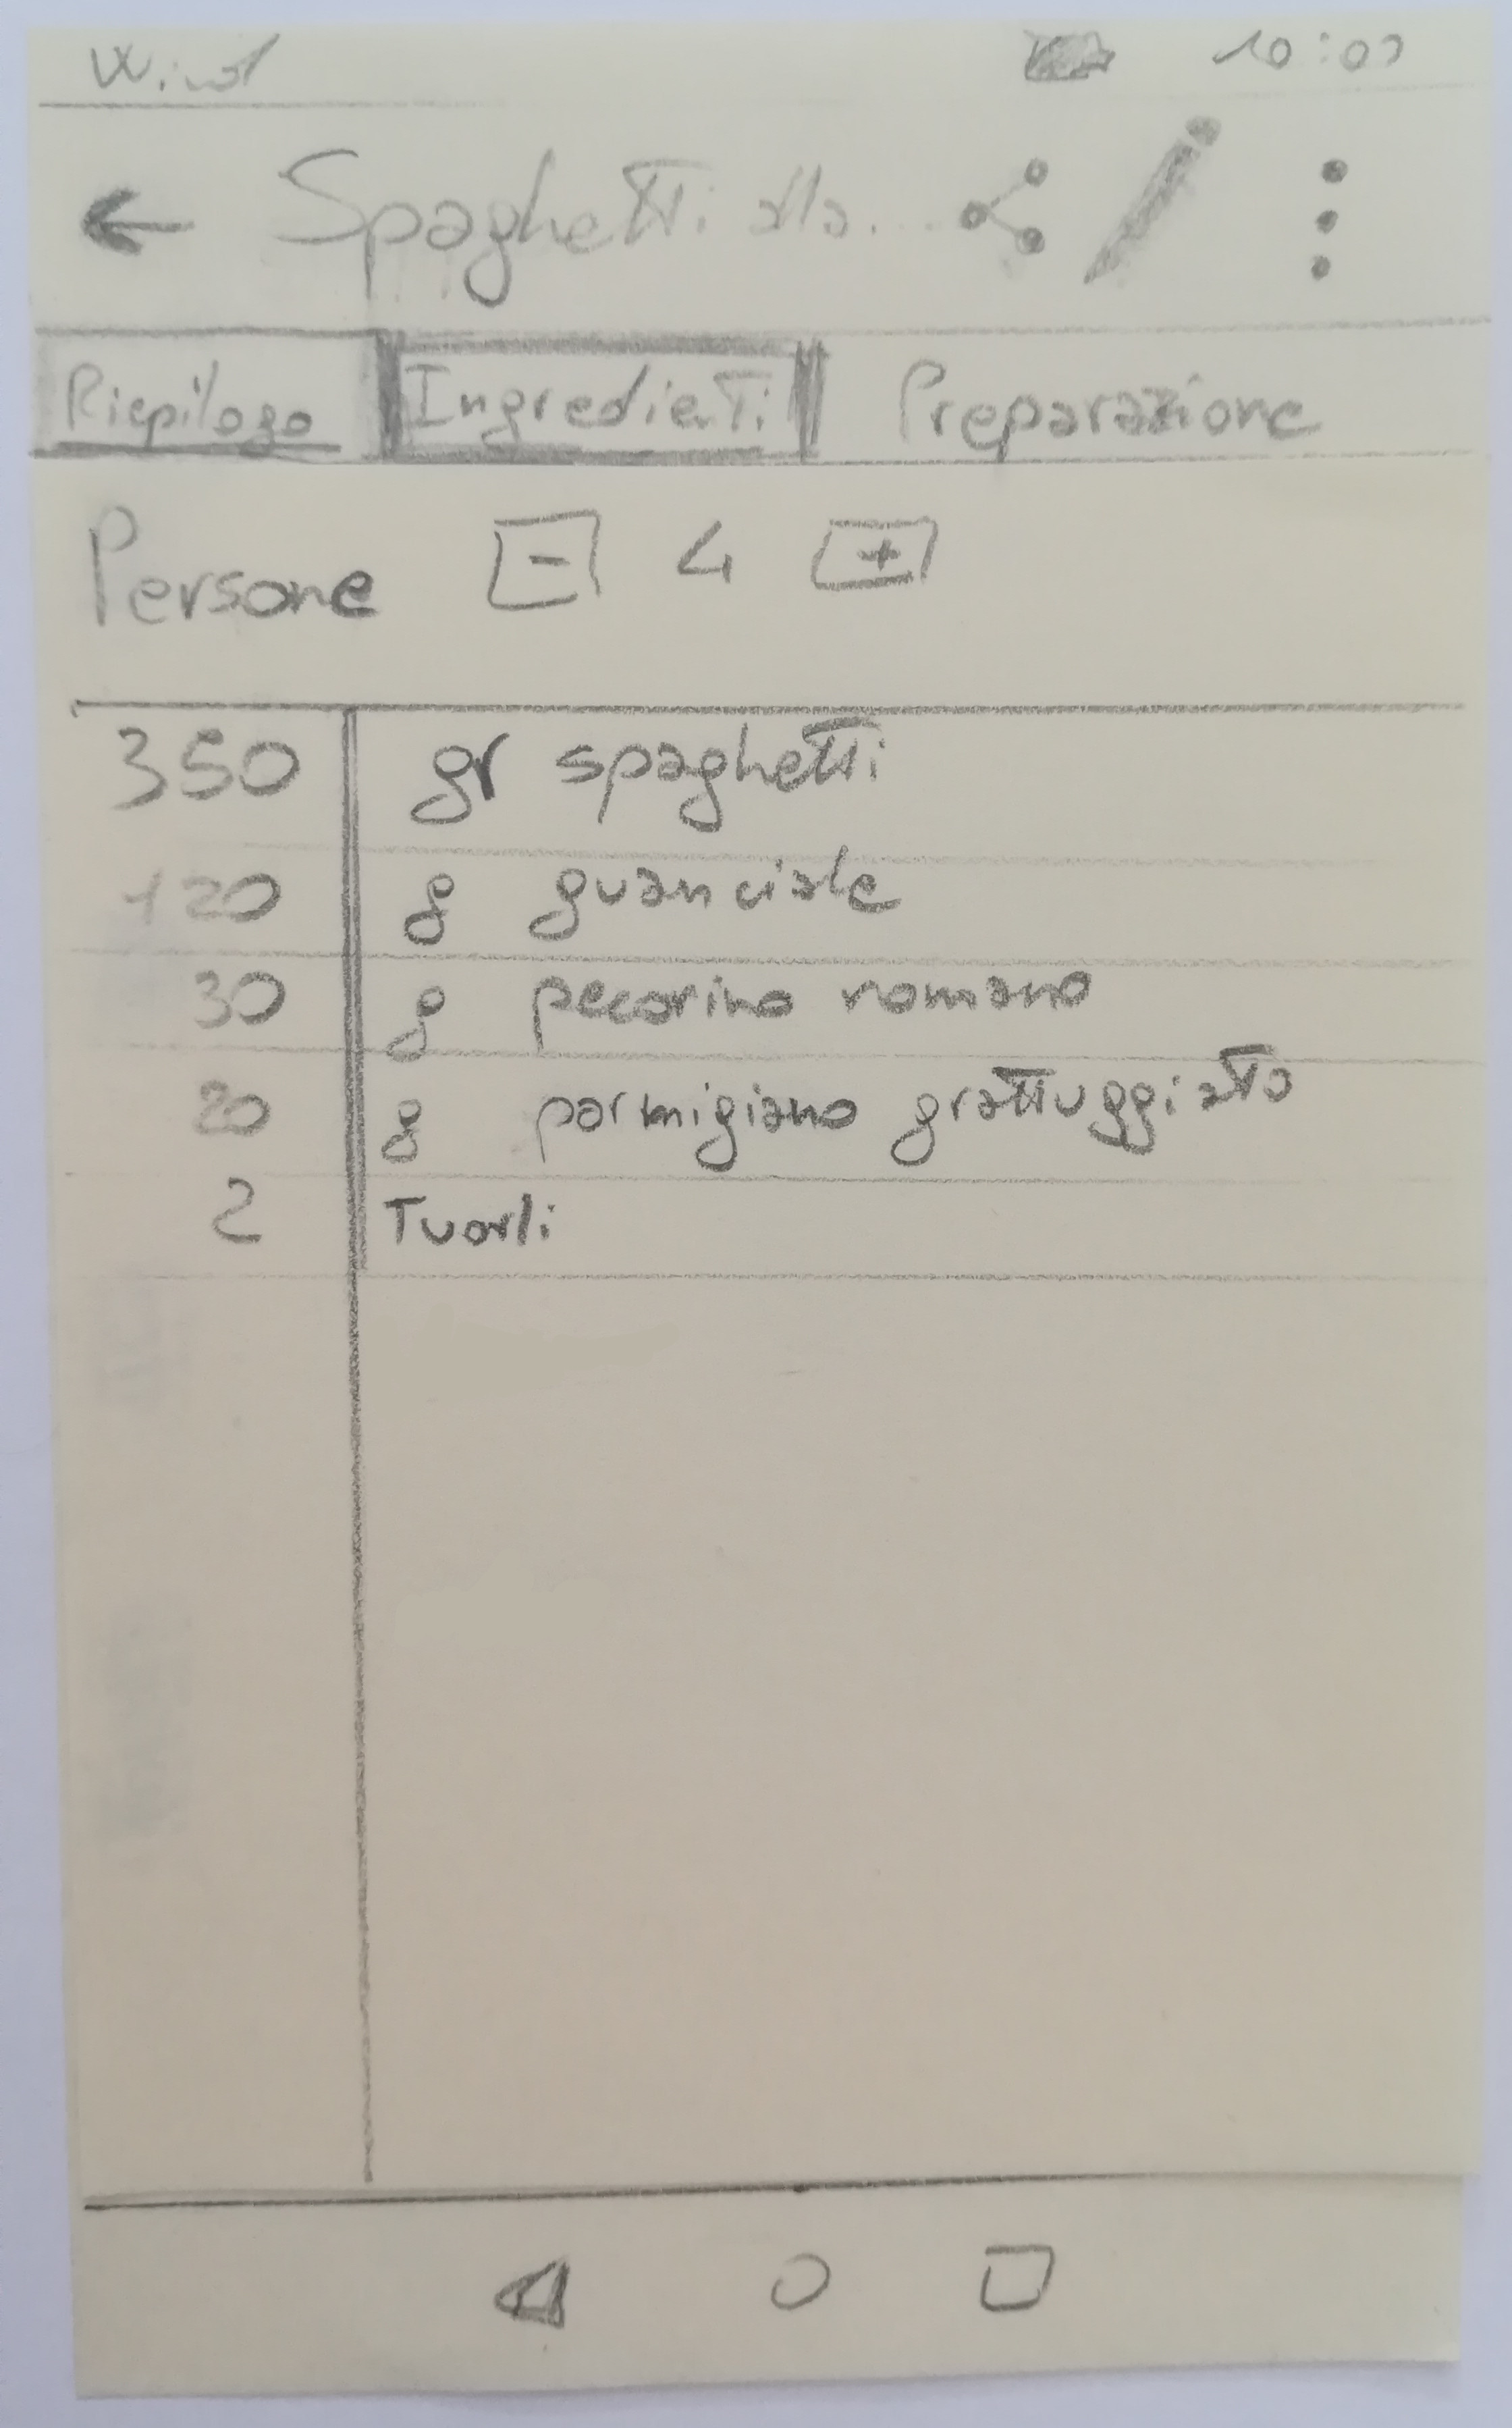
\includegraphics[width=0.4\textwidth]{prototipo1/ricetta_ingredienti}
    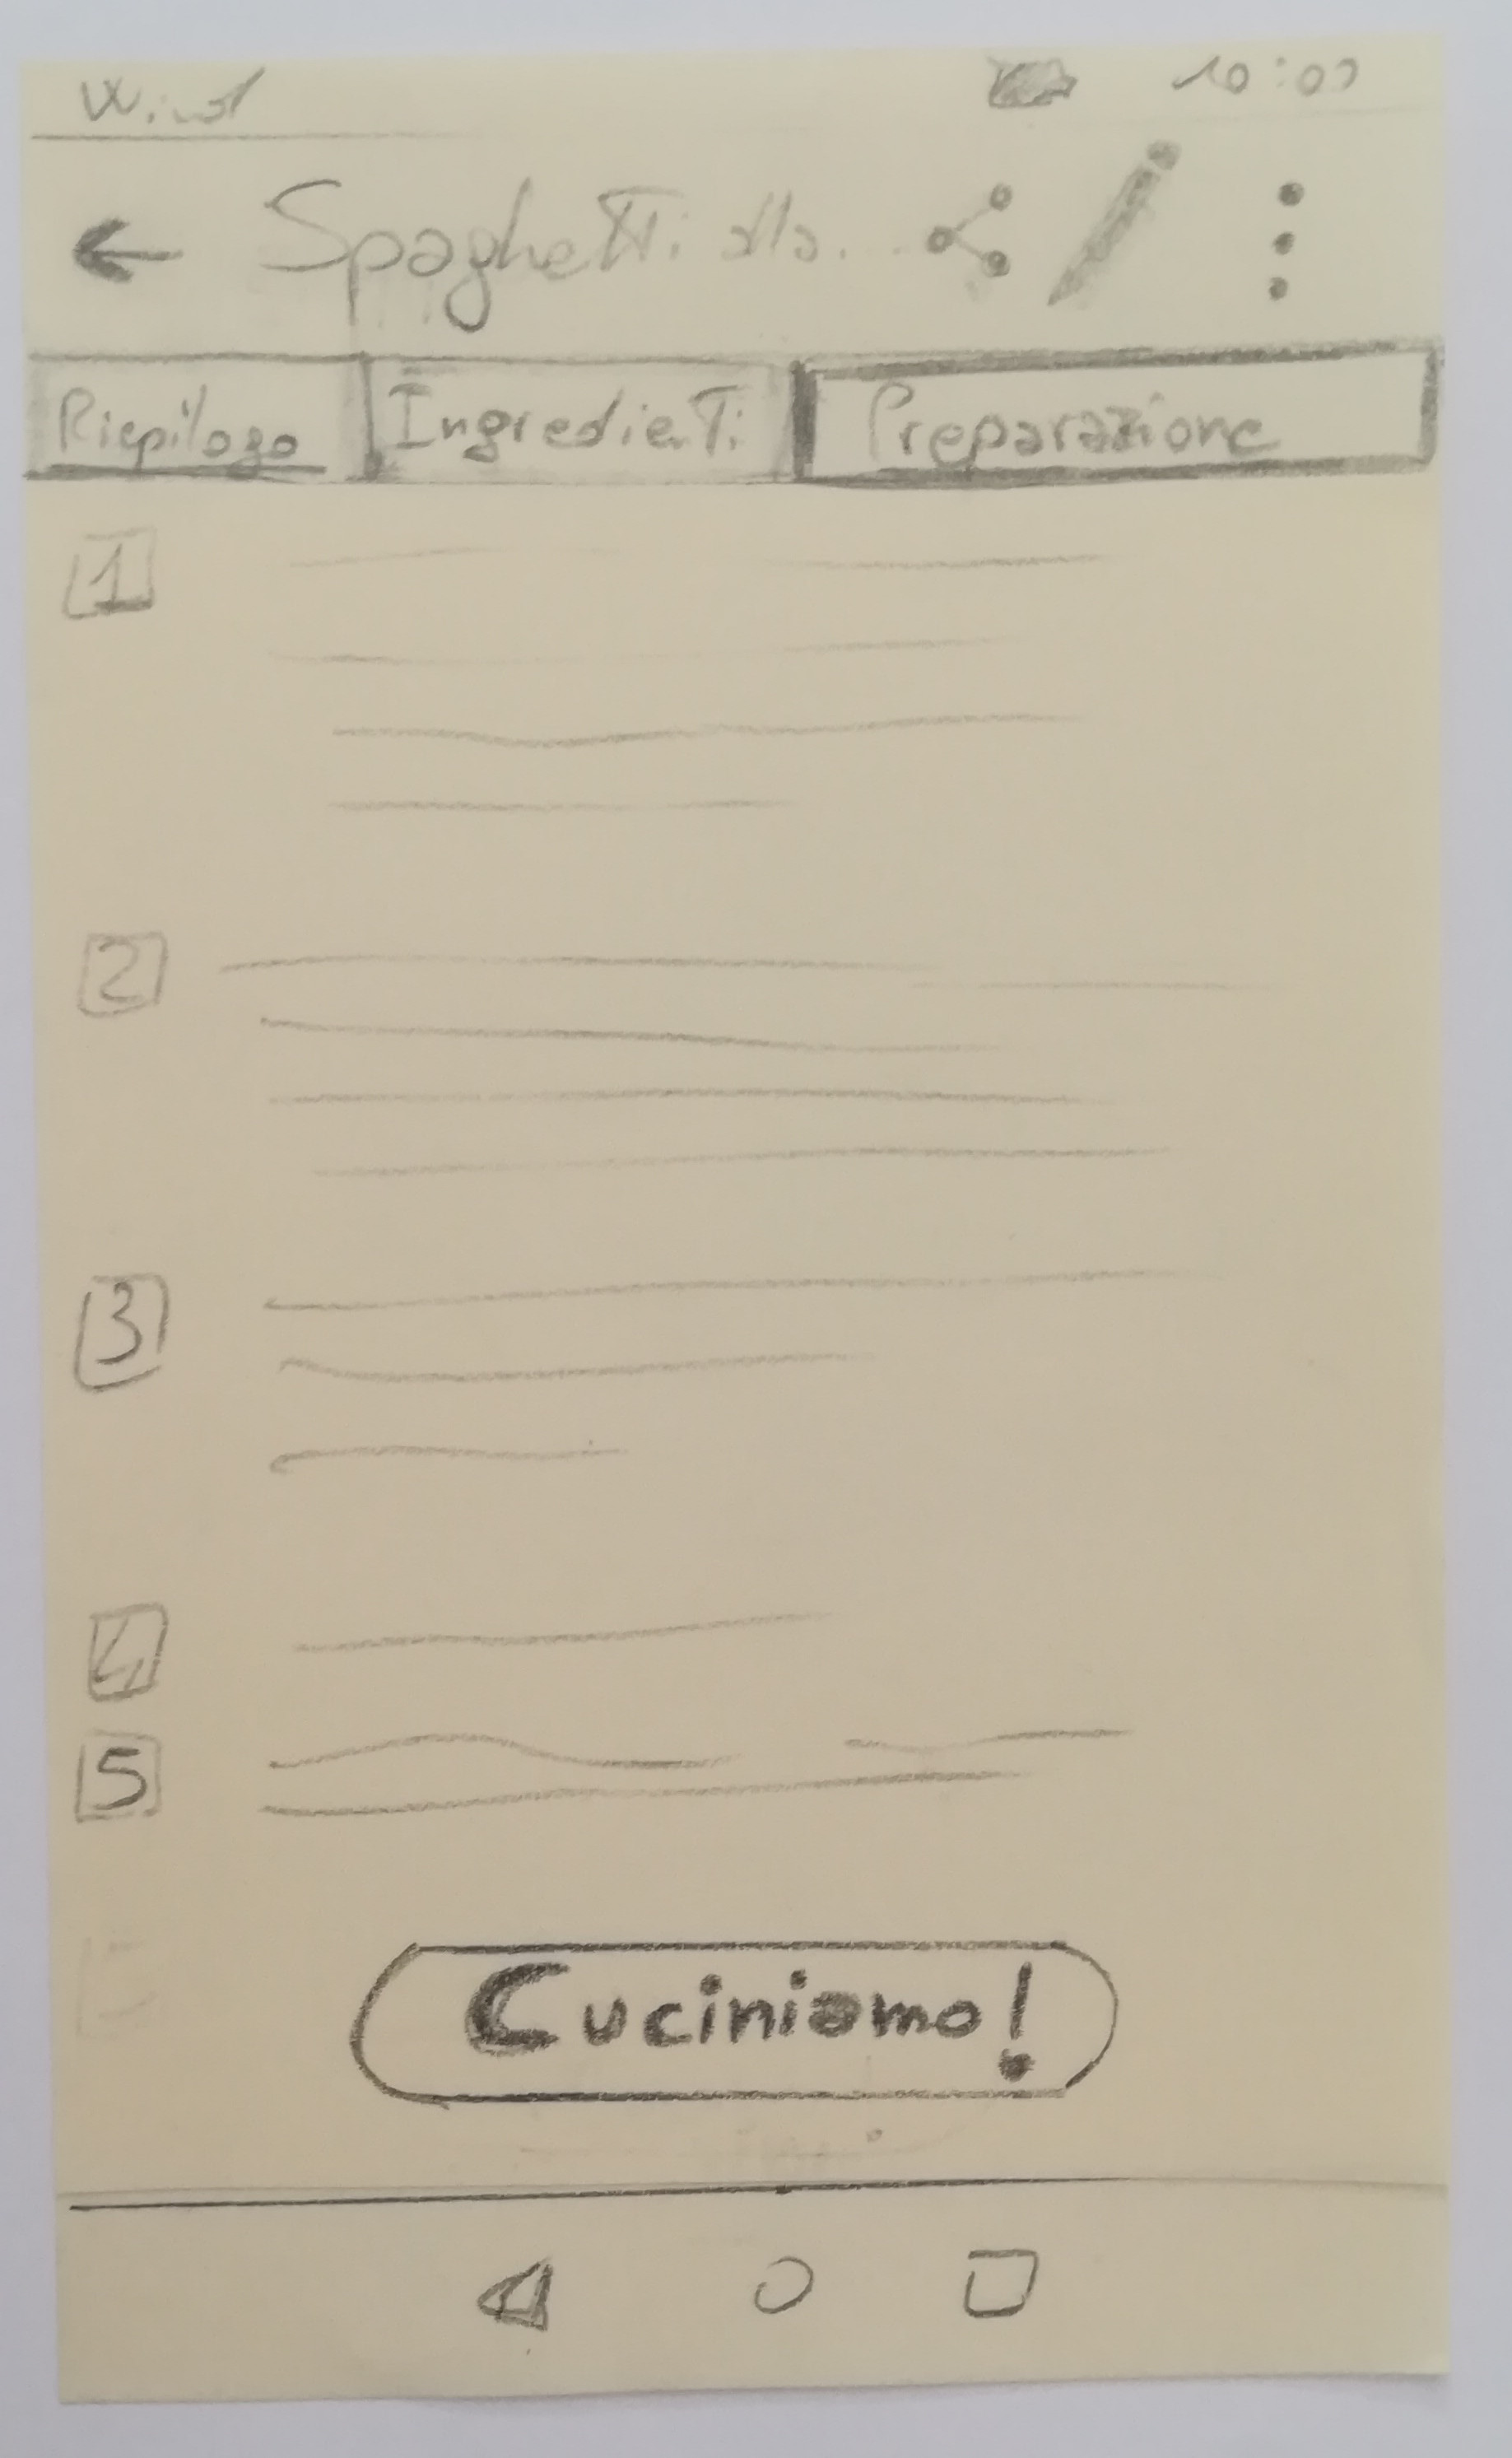
\includegraphics[width=0.4\textwidth]{prototipo1/ricetta_preparazione}
    \caption{Da sinistra a destra: }
    \label{fig:p1_ricetta}
  \end{center}
\end{figure}



\clearpage
\subsubsection{Descrizione del Design}
\subsubsection{Valutazione}

\subsection{Secondo Prototipo Low-Fidelity}
\subsubsection{Descrizione del Design}
\subsubsection{Valutazione}

\subsubsection{Design Alternativi}

\subsection{Conclusioni e Design Finale}
